\documentclass{book}

\usepackage[utf8]{inputenc}
\usepackage{titlesec}
\usepackage{easylist}
\usepackage{hanging}
\usepackage{hyperref}
\usepackage[a4paper,top=2.0cm,bottom=2.0cm,left=2.0cm,right=2.0cm]{geometry}
\usepackage{blindtext}
\usepackage{tipa}
\usepackage{epigraph}
\usepackage{enumerate}
\usepackage{longtable}
\usepackage{setspace}
\usepackage{verbatim}
\usepackage[T1]{fontenc}
\usepackage{graphicx}
\usepackage[italian]{babel}
\usepackage{amsmath}
\usepackage{pbox}
\usepackage{fancyhdr}
\usepackage{cancel}
\usepackage{tabularx}
\usepackage{booktabs}
\usepackage{multirow}
\usepackage{longtable}
\usepackage{tikz}
\usepackage{tikz-qtree}
\usepackage{subfig}
\usepackage{xcolor}
\usepackage{amssymb}
\usepackage{mathrsfs}
\usepackage{textcomp}
\usepackage{xfrac}
\usepackage{dsfont}

\usepackage{listings}
\usepackage{color}

\definecolor{mygreen}{rgb}{0,0.6,0}
\definecolor{mygray}{rgb}{0.5,0.5,0.5}
\definecolor{mymauve}{rgb}{0.58,0,0.82}

\lstset{ 
  backgroundcolor=\color{white},   % choose the background color; you must add \usepackage{color} or \usepackage{xcolor}; should come as last argument
  basicstyle=\footnotesize,        % the size of the fonts that are used for the code
  breakatwhitespace=false,         % sets if automatic breaks should only happen at whitespace
  breaklines=true,                 % sets automatic line breaking
  captionpos=b,                    % sets the caption-position to bottom
  commentstyle=\color{mygreen},    % comment style
  deletekeywords={...},            % if you want to delete keywords from the given language
  escapeinside={\%*}{*)},          % if you want to add LaTeX within your code
  extendedchars=true,              % lets you use non-ASCII characters; for 8-bits encodings only, does not work with UTF-8
  firstnumber=1000,                % start line enumeration with line 1000
  frame=single,	                   % adds a frame around the code
  keepspaces=true,                 % keeps spaces in text, useful for keeping indentation of code (possibly needs columns=flexible)
  keywordstyle=\color{blue},       % keyword style
  language=Octave,                 % the language of the code
  morekeywords={*,...},            % if you want to add more keywords to the set
  numbers=left,                    % where to put the line-numbers; possible values are (none, left, right)
  numbersep=5pt,                   % how far the line-numbers are from the code
  numberstyle=\tiny\color{mygray}, % the style that is used for the line-numbers
  rulecolor=\color{black},         % if not set, the frame-color may be changed on line-breaks within not-black text (e.g. comments (green here))
  showspaces=false,                % show spaces everywhere adding particular underscores; it overrides 'showstringspaces'
  showstringspaces=false,          % underline spaces within strings only
  showtabs=false,                  % show tabs within strings adding particular underscores
  stepnumber=2,                    % the step between two line-numbers. If it's 1, each line will be numbered
  stringstyle=\color{mymauve},     % string literal style
  tabsize=2,	                   % sets default tabsize to 2 spaces
  title=\lstname                   % show the filename of files included with \lstinputlisting; also try caption instead of title
}

\linespread{1.5} % l'interlinea

\frenchspacing

\newcommand{\abs}[1]{\lvert#1\rvert}

\usepackage{floatflt,epsfig}

\usepackage{multicol}
\newcommand\yellowbigsqcup[1][\displaystyle]{%
  \fboxrule0pt
  \ifx#1\textstyle\fboxsep-0.6pt\else\fboxsep-1.25pt\fi
  \mathrel{\fcolorbox{white}{yellow}{$#1\bigsqcup$}}}

\title{Formulario Fisica 1}
\author{Nicola Ferru}

% definizioni
\newtheorem{defi}{Definizione}[section]
\newtheorem{nota}{Nota}[section]

% stili grafici
\usepackage{tikzit}
\input{img/sstyle.tikzstyles}
\input{img/stile.tikzstyles}

\begin{document}
\maketitle
\tableofcontents

\chapter{Cinematica}
\label{sec:cin}

\section{Moto uniformemente accelerato}
\label{sec:motouniacc}

Formula per calcolare la Velocità finale:
\begin{equation}
  \label{eq:vf}
  V_f=v_0+a\cdot t
\end{equation}
di cui le singole variabili hanno il seguente significato:
\begin{itemize}
\item $v_0$ è la velocità di partenza;
\item $a$ è l'accelerazione;
\item $t$ è il periodo di tempo.
\end{itemize}
Mentre il sistem base del moto uniformemente accelerato è:
\begin{equation}
  \label{eq:motouniaccformbase}
  \begin{cases}
    v=v_i+a\Delta t\\
    s=\frac{1}{2}a(\Delta t)^2+v_i\Delta t+s_i
  \end{cases}
\end{equation}
o, in forma splicita
\begin{equation}
  \label{eq:motouniaccformbase2}
  \begin{cases}
    v=v_i+a(t-t_i)\\
    s=\frac{1}{2}a(t-t_i)^2+v_i(t-t_i)+s_i
  \end{cases}
\end{equation}
\subsection{Segmento percorso $s$ dopo il tempo $t$}
\label{sec:segPDTempt}
Per il parloco del segmento percorso $s$, se prendiamo come riferimento la perte dopo il tepo $t$, dobbiamo utilizzare:
\begin{equation}
  \label{eq:segperdopot}
  s=s_0+v_0\cdot t \pm \frac{a}{2}\cdot t^2
\end{equation}
Il segno dipende dal sistema di riferimento -- Le veriabili in gioco sono le seguenti:
\begin{itemize}
\item $s_0$ il segmento nel momento iniziale;
\item $v_0$ la velocità nel momento iniziale;
\item $a$ accelerazione;
\item $t$ il periodo di tempo.
\end{itemize}

\subsection{Velocità}
\label{sec:velmotouniformacc}
\begin{eqnarray}
  \label{eq:velmotouniformacc}
  v=v_i+a(t-t_i)
\end{eqnarray}

\begin{description}
\item[$v_i=$] velocità iniziale;
\item[$t_i=$] Tempo iniziale;
\item[$a=$] Accelerazione.
\end{description}

\subsection{Equazione senza il tempo}
\label{sec:eqsenzailtempo}

\begin{equation}
  \label{eq:eqsenzailtempo}
  v^2=v_0^2+2a(s-s_0)
\end{equation}
\subsection{Corpo che cade}
\label{sec:corpochecade}
\begin{equation}
  \label{eq:altezzadicaduta}
  h=h_0+v_0\cdot t \pm \frac{g}{2}\cdot t^2
\end{equation}
Il segno dipende dal sistema di riferimento -- le variabili in gioco sono:
\begin{itemize}
\item $h_0$ altezza nel momento iniziale;
\item $v_0$ la velocità nel momento iniziale;
\item $t$ il periodo di tempo;
\item $g$ forza peso.
\end{itemize}

\subsection{Caduta da $h_0$ con velocità iniziale nulla}
Le formule correlate ad un grave che cade da un altezza $h_0$ con una velocità $v_0=0$, sono le seguenti:
\label{sec:cadutadahconvelzero}
\begin{multicols}{2}
  \subsubsection{Tempo di caduta}
  \label{sec:tempcad}
  \begin{equation}
    \label{eq:tempcad}
    t_c=\sqrt{\frac{2h_0}{g}}
  \end{equation}
  \subsubsection{Velocità finale}
  \label{sec:velFin}
  \begin{equation}
    \label{eq:velfin}
    V_f=\sqrt{2gh}
  \end{equation}
\end{multicols}
Visto che la velocità conosciutà è quella iniziale che è nulla, all'interno delle formule sono presenti solamente l'altezza $h_0$ e la forza peso $g$.

\subsection{Lancio verso l'alto}
\label{sec:lancioversolalto}
Nel caso del lancio verso l'alto sono presenti queste due formule:
\begin{multicols}{2}
  \subsubsection{Altezza finale}
  \label{sec:altfinlancioversalt}
  \begin{equation}
    \label{eq:altfinlancioversalt}
    h=\frac{V_0^2}{2g}
  \end{equation}
  \subsubsection{Tempo finale}
  \label{sec:tempofinlancioveralt}
  \begin{equation}
    \label{eq:tempofinlancioveralt}
    t_h=\frac{V_0}{g}
  \end{equation}
\end{multicols}
In questo caso le variabile che entrano in gioco sono:
\begin{itemize}
\item La velocità $V_0$;
\item La forza peso $g$.
\end{itemize}

\section{Moto circolare uniforme}
\label{sec:motCircUni}
\begin{defi}
  Il moto circolare uniforme è il moto di un punto che percorre una traiettoria circolare (moto circolare) con velocità costante (moto uniforme). Velocità costante vuol dire che percorre archi di uguale lunghezza in intervallo di tempo uguale. La velocità si rappresenta un vettore tangente alla circonferenza (perpendicolare al raggio), vettore che ha modulo costante ma cambia continuamente direzione. \\
  L'accelerazione tangenziale, che è dovuta alle variazioni del modulo della velocità, è quindi nulla. L'accelerazione centripeta, che è dovua alle variazioni della direzione della velocità, non è nulla ed ha modulo costante. Il verso del moto circolare si dice orario se è concorde con quello delle lancette dell'orologio, antiorario in caso contrario.
  \begin{multicols}{2}
    \subsubsection{Accelerazione centripeta}
    \label{sec:acccent}
    \begin{equation}
      \label{eq:acccentripeta}
      a_c=\frac{V^2}{r}
    \end{equation}
    \subsubsection{Velocità angolare}
    \label{sec:velang}
    \begin{equation}
      \label{eq:velang}
      \omega=\sfrac{2\pi_{rad}}{T}=2\pi\cdot v
    \end{equation}
    \begin{equation}
      \label{eq:Velang}
      \omega = \frac{\Delta \alpha}{\Delta t}
    \end{equation}
  \end{multicols}
  $\Delta\alpha =$ angolo spezzato al centro
\end{defi}

\subsection{Energia cinetica totale}
\label{sec:encintot}

\begin{equation}
  \label{eq:encintot}
  E=\frac{1}{2} mv^2
\end{equation}

\subsection{Forza centripeta e centrifuga}
\label{sec:forzcentecentr}

\begin{multicols}{2}
  \subsubsection{Forza centripeta}
  \label{sec:forzacent}
  \begin{equation}
    \label{eq:forzacent}
    F_{CP}=m\cdot \frac{v^2}{r}
  \end{equation}
  
  \subsubsection{Forza centrifuga}
  \label{sec:forzacentrifuga}
  \begin{equation}
    \label{eq:forzacentrifuga}
    F_{CF}=-m\cdot\frac{v^2}{r}
  \end{equation}
\end{multicols}
Dato che le due formule danno due valori uno opposto all'altro possiamo dire senza ombra di dubbio che:
\begin{equation}
  \label{eq:equalscrcrnt}
  \boxed{F_{CP}=-F_{CF}}
\end{equation}
\begin{defi}
  Ogni lato di un triangolo rettangolo è maggiore della differenza degli altri due e minore della loro somma.
\end{defi}

\section{Somma dei vettori}
\label{sec:sommavect}
La somma dei vettori segue il seguente cruterio:
\begin{equation}
  \label{eq:sommavect}
  \abs{\vec{v}}=\sqrt{\abs{v_1}^2+\abs{v_2}^2+2\abs{v_1}\abs{v_2}+\log \alpha}
\end{equation}
La posizione e direzione di un vettore sono fondamentali per capire come essi agiscano. I tre casi più comuni sono:
\begin{description}
\item[Ortogonali] $\abs{v}=\sqrt{\abs{v_1}^2+\abs{v_2}^2}$
\item[Stessa direzione, vorso concorde] $\abs{v}=\abs{v_1}+\abs{v_2}$
\item[Stessa direzione, verso opposto] $\abs{v}=\abs{v_1}-\abs{v_2}$
\end{description}

\section{Prodotto tra vettori}
\label{sec:prodottotravect}

\subsection{Scalare}
\label{sec:scalare}

\begin{equation}
  \label{eq:scalare}
  a\cdot b=a\cdot\abs{b_p}
\end{equation}
Di cui $\abs{b_p}$ è il componente di $b//ad\text{ }a$
\begin{figure}[ht!]
  \centering
  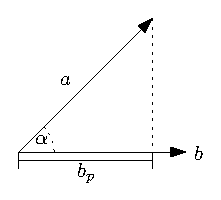
\includegraphics{img/scalare.eps}
  \caption{prodotto vettoriale scalare}
  \label{fig:prodvectscal}
\end{figure}
\begin{equation}
  \label{eq:scalare2}
  a\cdot b= a\cdot b\cdot \cos \alpha
\end{equation}

\subsection{Vettoriale}
\label{sec:vectprod}
\begin{equation}
  \label{eq:prodvec}
  \begin{matrix}
    a\cdot b=a\cdot b\cdot \sin \alpha & a_n \dot b
  \end{matrix}
\end{equation}
di cui, $a_n$ è componente di $a \bot a b$.

\section{Moto con accelerazione variabile}
\label{sec:motoconaccevar}

\subsection{Velocità dopo un tempo $t$}
\label{sec:veldopotempt}
\begin{equation}
  \label{eq:veldopuntemptacvar}
  v=v_0+\int^t_{t_0}a(t)dt
\end{equation}
In questo caso ci le variabili in gioco sono:
\begin{itemize}
\item $t_0\to$ interno iniziale;
\item $v_0\to$ velocità iniziale.
\end{itemize}
Questa formula è anche chiamata ``integrale dell'accelerazione rispetto al tempo'' -- equivale sempre all'area sotto al grafico $a(t)-t$.
\begin{center}
  accelerazione = derivata rispetto al tempo $\Leftrightarrow$ Velocità = integrale di $a(x)$ in $dt$
\end{center}

\subsection{Forza di attrito}
\label{sec:forzadiattr}
\begin{multicols}{2}
  \subsubsection{Attrito statico}
  \label{sec:attrstatico}
  \begin{equation}
    \label{eq:attrstatico}
    fs=\mu_sN
  \end{equation}
  
  \subsubsection{Attrito dinamico}
  \label{sec:attrdinamico}
  \begin{equation}
    \label{eq:attrdinamico}
    f_k=\mu_kN
  \end{equation}
\end{multicols}
Forza che si origina quando due campi a contatto diretto sono fatti souegare uno con l'altro.
\begin{itemize}
\item $N=$ forza normale esercitata dal piano (\textit{appena alla forza peso})
\item $\mu_s=$ Coefficiente di attrito statico;
\item $\mu_s=$ Coefficiente di attrito dimamico.
\end{itemize}
\begin{nota}
  L'attrito statico ha un valore massimo generalmente più alto rispetto a quello dinamico. Quando un corpo è meno da una forza $F$, se $F=f_k$ il corpo \textsc{si muove a velocità Costante}. 
\end{nota}

\section{Piano inclinato}
\label{sec:pianoinclinato}

\begin{multicols}{2}
  \subsubsection{Accelerazione perpendicolare al piano}
  \label{sec:accperpalpiano}
  \begin{equation*}
    a_y=0
  \end{equation*}
  
  \subsubsection{Accelerazione parallela al piano}
  \label{sec:accparalpiano}
  \begin{equation*}
    a_x=g\cdot \sin(\alpha)
  \end{equation*}
  in cui $g$ è la forza di gravità, mentre, $\alpha$ è l'angolo del piano.
  
  \subsubsection{Angolo d'altezza e lunghezza}
  \label{sec:angolodaltelung}
  \begin{equation*}
    \sin(\alpha)=\frac{h}{l}
  \end{equation*}
  
  \subsubsection{Angolo da base e lunghezza}
  \label{sec:angdabaseelungh}
  \begin{equation*}
    \cos(\alpha)=\frac{d}{l}
  \end{equation*}
  
  \subsubsection{Angolo d'altezza e base}
  \label{sec:angdaltebase}
  \begin{equation*}
    \tan(\alpha)=\frac{h}{d}
  \end{equation*}
\end{multicols}

\clearpage
\section{Moto Parabolico (Moto del proiettile)}
\label{sec:motoparabolico}

\begin{defi}
  Un \textbf{moto parabolico} è il moto di un corpo che, partendo con una certa velocità iniziale e un certo angolo, percorre una traiettoria parabolica sotto l'azione della sola accelerazione di gravità.
\end{defi}
\begin{figure}[ht!]
  \centering
  \resizebox{4cm}{!}{
    \begin{tikzpicture}
	\begin{pgfonlayer}{nodelayer}
		\node [style=none] (0) at (0, 6) {};
		\node [style=none] (1) at (0, 0) {};
		\node [style=none] (2) at (7, 0) {};
		\node [style=none] (3) at (0, 0) {};
		\node [style=none] (4) at (0.5, -0.5) {$\vec{V}_{0x}$};
		\node [style=none] (5) at (-0.75, 1.25) {$\vec{V}_{0y}$};
		\node [style=none] (6) at (0, 2) {};
		\node [style=none] (7) at (1, 0) {};
		\node [style=none] (8) at (1, 2) {};
		\node [style=none] (9) at (6.5, 0) {};
		\node [style=none] (10) at (6.5, -0.5) {$X$};
		\node [style=none] (11) at (1, 2.5) {$\vec{V}_0$};
		\node [style=none] (12) at (-0.5, 5.75) {$Y$};
	\end{pgfonlayer}
	\begin{pgfonlayer}{edgelayer}
		\draw [style=Rightarrow] (1.center) to (0.center);
		\draw [style=Rightarrow] (3.center) to (2.center);
		\draw [style=Rightarrow] (3.center) to (7.center);
		\draw [style=Rightarrow] (3.center) to (6.center);
		\draw [style=Rightarrow] (3.center) to (8.center);
		\draw [style=DashedCampitura] (6.center) to (8.center);
		\draw [style=DashedCampitura] (8.center) to (7.center);
		\draw [style=campitura, bend left=60, looseness=1.75] (3.center) to (9.center);
	\end{pgfonlayer}
\end{tikzpicture}

  }
  \caption{Moto parabolico}
  \label{fig:motopar}
\end{figure}
Per ricavare i componenti di $V_0$, si utilizza la trigonometria, infatti, mettendo tutto in forma sistemica il risultato è il seguente:
\begin{equation}
  \label{eq:componentixymotopar}
  \begin{cases}
    v_{0x}=v_0\cos(\alpha)\\
    v_{0y}=v_0\sin(\alpha)
  \end{cases}
\end{equation}
Per questo mtivo per ottenere la velocità può essere utilizzato il teorema di pitagora:
\begin{equation*}
  v=\sqrt{v_{0x}^2+v_{0y}^2}
\end{equation*}
Tramite $v_{0x}^2$ e $v_{0y}^2$ è possibile essere anche utilizzato per ricavare la tangente:
\begin{equation*}
  \tan(\alpha)=\frac{v_{0x}}{v_{0y}}
\end{equation*}
L'equazione parametrica base invece è definita da due cordinete (\textit{x} e \textit{y}):
\begin{equation}
  \label{eq:eqbasemotopar}
  \begin{cases}
    x=x_0+v_{0x}t\\
    y=-\frac{1}{2}gt^2+v_{0y}t+y_0
  \end{cases}
\end{equation}
Per ricavare il tempo, sarà invece necessario:
\begin{equation}
  \label{eq:tempomotopar}
  t=\frac{v_0\sin(\alpha)\pm \sqrt{v_0^2\sin^2(\alpha)+2gy_0}}{g}
\end{equation}

\subsection{Traiettoria del moto parabolico}
\label{sec:traietmotopar}

Per calcolare la traiettoria è necessario mettere il tempo $t$ e lo spazio $y$ è necessario:
\begin{eqnarray}
  \label{eq:traietdelmotopar}
  \begin{cases}
    t=\frac{x-x_0}{v_{0x}}\\
    y=-\frac{1}{2}gt^2+v_{0y}t+y_0
  \end{cases} & \text{(Oppure in forma esplicita)} & \begin{cases}
    t=\frac{x-x_0}{v_{0x}}\\
    y=-\frac{1}{2}g\left(\frac{x-x_0}{v_{0x}}\right)^2+v_{0y}\left(\frac{x-x_0}{v_{0x}}\right)+y_0
  \end{cases}
\end{eqnarray}

\chapter{Dinamica}
\label{chap:Dinamica}

\section{Lavora}
\label{sec:lavoro}

\subsection{Forza costante}
\label{sec:forcostlav}

\begin{defi}
  Il lavoro è il prodotto scalare tra la forza applicata ad un corpo e l spostamento compiuto da essa.
  \begin{equation}
    \label{eq:lavoro}
    L=(F\cdot \cos \alpha) \Delta s
  \end{equation}
  \begin{itemize}
  \item $F=$ modulo del vettore forza;
  \item $\Delta s=$ spostamento lungo un asse;
  \item $\alpha=$ angolo tra forza e spostamento.
  \end{itemize}
  quello che mai moltiplicano allo spostamento è {\color{red}la componente del vettore forza \textsc{parallela allo spostamento}}, dunque:
  \begin{eqnarray*}
    \text{>se } \alpha = 0, \Rightarrow L = F\cdot \Delta s & \text{\color{red}Forza parallela a spostameto}\\
    \text{>se } \alpha = 90^o, \Rightarrow L = 0 & \text{\color{red}Forza perpendicolare a spostamento} 
  \end{eqnarray*}
\end{defi}

\subsection{Forza variabile}
\label{sec:forzavarlav}
\begin{equation}
  \label{eq:forzavarlav}
  L_{1,2}=\int_{x_1}^{x_2}F(x)dx
\end{equation}
\begin{description}
\item[$x_{1,2}$ =] delimitano lo spazio entro cui vogliamo conoscere il lavoro compiuto da $F(x)$. 
\end{description}
Il lavoro compiuto da una forza è uguale all'asse sotto al grafico $F(x)-x$

\subsubsection{Unità di misura}
\label{sec:joule}

\begin{equation}
  \label{eq:joule}
  1N\cdot 1m=1J \textbf{ (Joule)}
\end{equation}

\subsection{Lavoro istantaneo}
\label{sec:lavoroistantaneo}

\begin{equation}
  \label{eq:lavista}
  dL=(F\cdot \cos \alpha)ds
\end{equation}
\begin{description}
\item[$ds=$] spostamento infinitesimo
\end{description}
\begin{nota}
  Se la forza cambia esclusivamente la direzione della velocità (\textit{e non il modulo}) \textsc{non compie lavoro}.
\end{nota}

\section{Potenza}
\label{sec:potenza}

\begin{defi}
  la potenza è il rapporto tra il lavoro compiuto da una forza e il tempo da essa compiendo per compierlo
\end{defi}
\begin{multicols}{2}
  \subsubsection{Potenza media}
  \label{sec:potmedia}
  \begin{equation}
    \label{eq:potmedia}
    <P>=\frac{\Delta L}{\Delta t}
  \end{equation}
  
  \subsubsection{Potenza istantanea}
  \label{sec:potistant}
  \begin{equation}
    \label{eq:potistant}
    P=\frac{dL}{dt}
  \end{equation}
\end{multicols}
\begin{itemize}
\item Se la pontenza è costante:
  \begin{equation}
    \label{eq:potconst}
    L=P\Delta t
  \end{equation}
\item Unità di misura:
  \begin{equation}
    \label{eq:unitadimisura}
    \frac{1 Joule}{1s}=1W
  \end{equation}
\end{itemize}

\section{Energia cinetica}
\label{sec:energiacin}

\begin{defi}
  L'energia cinetica è uguale al lavoro necessario per portare $m$ alla velocità $v$ (o al lavoro che la massa necessita per fermarsi)
  \begin{equation}
    \label{eq:energiacin}
    k=\frac{1}{2} mv^2
  \end{equation}
  \begin{itemize}
  \item $m=$ massa;
  \item $v=$ velocità.
  \end{itemize}
\end{defi}

\subsection{Teorema Lavoro-Energia}
\label{sec:teoLavEn}

\begin{equation}
  \label{eq:teoLavEn}
  L=k-k_0
\end{equation}
\begin{description}
\item[$L=$] lavoro totale della forza \textsc{Risultante}
\item[$k=$] Energia cinetica finale
\item[$k_0=$] Energia cinetica iniziale
\end{description}
Il lavoro svolto da una forza in una particella è uguale alla sua variazione di energia cinetica.
\begin{itemize}
\item Questo teorema permette di traciare il lavoro anche quando la forza non varia solo in modulo, \textsc{senza nessun integrale}. 
\end{itemize}

\subsection{Forze conservative e non conservative}
\label{sec:forconsenon}
\begin{itemize}
\item Conservative
  \begin{itemize}
  \item Durante il moto si conserva l'energia meccanica
  \item Il lavoro dipende solo dalla spostamento totale
  \item Il lavoro nello spostare un corpo lungo oercirsi kuberi è 0
  \end{itemize}
\item Non conservative
  \begin{itemize}
  \item Durante il moto \textsc{Non} si conserva l'energia meccanica;
  \item Il lavoro dipende dal percorso;
  \item Il lavoro dipende anche dal percorso effettuato. 
  \end{itemize}
\end{itemize}
I sostanza, una forza è conservativa se:
\begin{itemize}
\item Il lavoro da essa eseguito nello spostare un corpo dipede solo dallo spostamento totale, \textsc{Non} dal percorso.
\item Il lavoro da esso compiuto nello spostare un corpo lungo una linea chiusa è nullo (l'energia cinetica tarna la stessa di prima)
  \begin{equation*}
    L=\Delta k=0
  \end{equation*}
\end{itemize}

\subsubsection{Ricora}
\label{sec:ricLavposandNeg}
\begin{center}
  Lavoro Positivo $\Longleftrightarrow$ Aumenta energia cinetica\\
  Lavoro Negativa $\Longleftrightarrow$ Diminuisce energia cinetica
\end{center}

\section{Energia Potenziale}
\label{sec:enpot}

\begin{defi}
  L'energia potenziale si può definire soltanto quando abbiamo a che fare con una forza conservativa, che nel moto unidirezionale dipedono solo dalla posizione
  \begin{equation}
    \label{eq:enpot}
    \Delta k=-\Delta U
  \end{equation}
  \begin{description}
  \item[$\Delta k=$] variazione energia cinetica
  \end{description}
  a una variazione di $k$, ne corrisponderà una in senso apposto di $U$
  \begin{equation}
    \label{eq:differenzak}
    k_x-k_{x_0}=-(U_x-U_{x_0})
  \end{equation}
\end{defi}

\section{Energia meccanica}
\label{sec:enmecc}

\begin{equation}
  \label{eq:enmecc}
  E=k+U
\end{equation}
\begin{itemize}
\item $k=$ energia cinetica
\item $U=$ energia potenziale
\end{itemize}

\subsection{Legge di conservazione dell'energia meccanica}
\label{sec:leggconsenmec}

\begin{defi}
  Quando il moto cousato da una forza conservativa, l'energia meccanica si \textsc{Conserva} sempre
  \begin{itemize}
  \item al decrescere dell'energia cinetica, aumento l'energia potenziale e viceversa, {\color{red}dunque la somma rimane costante}.
    \begin{equation}
      \label{eq:leggconsenmec}
      k_0+U_0=k_F+U_F
    \end{equation}
  \end{itemize}
\end{defi}
\begin{multicols}{2}
  \begin{equation*}
    \Delta U=-\int_{x_0}^xF(x)dx
  \end{equation*}
  l'energia potenziale è una funzione di posizione la cui derivata (\textsc{conbiata di segno}) da la forza.\\
  \begin{equation*}
    F(x)=-\frac{dU(x)}{dx}
  \end{equation*}
  la forza (\textsc{cambiata di segno}) rappresenta la rapidità con cui l'energia potenziale varie lungo $x$.
\end{multicols}

\subsection{Energia potenziale gravitazionale}
\label{sec:enpotgrav}
\begin{equation}
  \label{eq:enpotgrav}
  U_y-U_0=mgy\\
  U(y)=mgy
\end{equation}
\begin{description}
\item[$y=$] posizione sull'asse verticale;
\item[$g=$] $9.8\sfrac{m}{s^2}$ oppure $9.81\sfrac{m}{s^2}$ dipende da diversi fattori
\item[$m=$] massa
\end{description}
\begin{equation*}
  U_y-U_0=\int_y^0F(y)dy=\int_y^0(-mg\cdot y)=mgy
\end{equation*}

\subsection{Energia potenziale elastica}
\label{sec:enerpotela}

\begin{equation*}
  U(x)=\int_x^0(-kx)dx=\frac{1}{2}kx^2
\end{equation*}

\subsection{Forza non conservative}
\label{sec:forzanoncon}

\begin{equation*}
  L_{non-cons.}=\Delta{}(k+U)=\Delta{}E
\end{equation*}
la presenza di forza non conservative comporta una variazione dell'energia meccanica totale del sistema
\begin{itemize}
\item Il teorema lavoro energia può essere scirtto come:
  \begin{equation*}
    L_{non-cons.}=\Delta{}k+\sum\Delta{}U
  \end{equation*}
\end{itemize}
\begin{description}
\item[$\sum\Delta U$] contributo di tutte le forze conservative presenti
\end{description}

\subsection{Legge di conservazione dell'energia}
\label{sec:leggconsen}
\begin{defi}
  L'energia totale di un sistema isolato, che risulta dalla somma di tute le forme di energia in esso presenti (Cinetica, potenziale, etc\dots) non cambia mai.
  \begin{itemize}
  \item questo ``teorema'' in realtà non ho una dimostrazione matematica, ma è verificato dalla semplice esperienza (non si è mai riscontrato un caso in cui questo principio non sia valido)
  \item matematicamente, il principio è valido fintanto che teniamo conto di ogni frma di energia presente nel sistema.
  \item Se l'energia meccanica non si conserva, essa è stata in altre forme (l'attrito la dissipa in calore).
  \end{itemize}
\end{defi}

\subsection{Centro di massa}
\label{sec:centdimassa}

Coordinata su un solo asse (del centro di massa di un sistem di n particelle)
\begin{equation}
  \label{eq:centdimassa}
  x_{cm}=\frac{\sum m_ix_i}{\sum m_i}
\end{equation}
\begin{itemize}
\item $\sum m_ix_i=$ sommatoria delle masse di ogni particella moltiplicate per la loro porzione in un asse;
\item $\sum m_i=$ massa totale del sistema.
\end{itemize}
Il centro di massa è del tutto indipendnete dal sistema di coordinate usato, ma dipende solo dalle distanze relative tra le particelle e dalle toro mane.
\begin{itemize}
\item È adattabile solo quando si ha $\alpha$ che fare con il moto \textsc{traslatorio};
\item È una sorta di media pounderata.
\end{itemize}
Nel caso di 2 o 3 dimensioni, si calcolano separatamente le coordinate del centro di massa in ogni asse con la stessa formula.

\subsubsection{coordinate centro di massa (carpo esteso e di materia uniforme)}
\label{sec:coordcentdimassa}

\begin{equation}
  \label{eq:coordcentdimassa}
  x_{cm}=\lim\limits_{\Delta m_i\to 0}= \frac{\sum m_ix_i}{\sum m_i}
\end{equation}
\begin{description}
\item[$m=$] massa totale del corpo
\end{description}
\begin{equation*}
  x_{cm}=\frac{\int x dm}{\int dm}=\frac{1}{M}\cdot \int x dm
\end{equation*}
\textsc{Fai lo stesso calcolo su tutti gli assi presenti}
\begin{center}
  Centro di massa = Baricentro
\end{center}

\subsubsection{Equazione vettoriale del centro di massa}
\label{sec:eqvettdelcentrodimassa}

\begin{equation}
  \label{eq:eqvettdelcentrodimassa}
  \vec{s}_{cm}=\frac{\int \vec{s}dm}{\int dm}
\end{equation}
\begin{description}
\item[$\vec{s}=$] vettore posizione 
\end{description}
Tieni a mente che molti dei carpi che potresti deve trattare sono dettati di assi, punti o piani di {\color{red}simmetria}, uniti per individuare il centro di massa (in quel punto, lungo quella linea, \dots).

\subsubsection{Accelerazione del centro di massa (di un sistema di particelle)}
\label{sec:accdelcentrodimass}
\begin{equation}
  \label{eq:accdelcentrodimass}
  M_{cm_x}=\sum F_i = \sum m_i\frac{dV_{i_x}}{dt}
\end{equation}
Il prodotto della massa complessivo del gruppo di particelle per l'accelerazione del centro di massa è uguale alla somma vettariale di tutte le forze che agiscono sul sistema di sistema di porticella (\textsc{incluse quelle interne}).

\subsubsection{Legge del moto traslatorio del centro di massa}
\label{sec:leggedelmottrasldelcndimassa}
\begin{equation}
  \label{eq:leggedelmottrasldelcndimassa}
  F_{est}=Ma_{cm}
\end{equation}
\begin{description}
\item[$f_{est}=$] risultante forza esterne;
\item[$M=$] massa totale sistema;
\item[$a=$] accelerazione centro di massa.
\end{description}
\begin{nota}
  Qualsiasi sia il sistema di particelle e qualsiasi configurazione esso abbia, esso si muoverà sempre secondo questa legge.
\end{nota}

\subsection{Quantità di moto}
\label{sec:quantmoto}

\begin{equation}
  \label{eq:quantmoto}
  \vec{P}=mv
\end{equation}
Parte a una nuova difinizione per la forza:
\begin{equation*}
  \vec{F}=\frac{d\vec{P}}{dt}
\end{equation*}
$F=ma$ infatti, è utilizzabile solo se la massa è costante.
\begin{itemize}
\item La quantità di moto totale di un sistema equivale alla somma \textsc{Vettoriale} di tutte le quantità di moto;
\item Quantità di moto totale di un sistemaç massa totale $\cdot$ velocità centro di massa:
  \begin{equation*}
    P_{Tot}=M\cdot V_{cm}
  \end{equation*}
\end{itemize}
La quantità di moto di un sistem isolato \textsc{si conseva}, in quanto non subisce forze esterne. (viceversa, la quantità di moto può essere variata solo da forze esterne al sistema).
\begin{itemize}
\item le quantità di massa della singole particelle possono variare, ma non in totale
\end{itemize}
\begin{equation*}
  \frac{d\vec{P}}{dt}=F_{ext}
\end{equation*}
Il tempo di variazione della quantità di moto totale di un sistema di particelle è dato dalla rosiltante di tutte le forze esterne applicate al sistema.
\begin{eqnarray*}
  \vec{F}=\frac{d\vec{P}}{dt} & \text{Forza (istantanea)} = \frac{\text{variazione di quantità di moto (infinitesimo)}}{\text{Variare del tempo (infinitesimo)}}
\end{eqnarray*}
\paragraph{Enuncia questo se chiede la seconda legge di Newton}
Condizioni per il moto di un sistema:
\begin{center}
  Conservazione energetica \textrightarrow{} 1 (scalabile)\\
  Conservazione quantità di moto \textrightarrow{} 3 (vettoriale, un equazione per ogni coordinata)
\end{center}

\paragraph{Forza impulsiva:}

Agisce in tempo brevissimi con un intensità molto elevata, di solito riscontrata negli urti (\textsc{Internità varia nel tempo})

\subsection{Teorema dell'impulso -- quantità di moto}
\label{sec:teodelimpquantmoto}
\begin{eqnarray}
  \label{eq:teoremadelimp}
  \vec{J}=\int_{t_1}^{t_2}F(t) dt=\Delta P
\end{eqnarray}
\begin{description}
\item[$J=$] ``impulso'';
\item[$\Delta P=$] Variazione quantità di moto.
\end{description}
La variazionem di quantità di moto cui è sottoposto un corpo in cui agisce una forza impulsiva è uguale all'inpulso.
\begin{itemize}
\item L'impulso è un vettore il cui modulo equivale all'asse sotto al grafico $F(t)-t$
\item La direzione dov'essere costante.
\end{itemize}

\subsubsection{Urti}
\label{sec:urti}
\begin{description}
\item[Elastici] L'energia cinetica (totale) si conserva e la quantità di moto si conserva;
\item[Anaelastici] L'energia cinetica non si conserva e la quantità di moto si conserva;
\item[Completamente anelastici] corpi rimangorno attaccati
\end{description}

\subsection{Urto elastico a 2 dimensioni}
\label{sec:urtela2dim}
\begin{equation}
  \label{eq:urtela2dim}
  V_1+V_1=V_2+V_2
\end{equation}
\begin{nota}
  la velocità della massa1 resta uguale prima e dopo l'urto esattamente come succede nel caso della massa2.
\end{nota}
\begin{equation}
  \label{eq:differenzatravel}
  V_1-V_2=V_2-V_1
\end{equation}
Le differenze di velocità di ognuno delle masse prima e dopo l'urto sono uguali e contrarie
\begin{equation*}
  \frac{1}{2}m_1V_1^2+\frac{1}{2}m_2V_2^2=\frac{1}{2}m_1V_1^2+\frac{1}{2}m_2V_2^2
\end{equation*}
Per ottenere le velocità, metti a sistema questa equazione con quella in cima.

\subsubsection{Velocità urto completamente anelastico}
\label{sec:velurtocompan}
\begin{equation}
  \label{eq:velurtcompan}
  m_1V_1+m_2V_2=(m_1+m_2)V
\end{equation}

\section{Moto rotatorio}
\label{sec:motorot}

\subsection{Misura angolo in radianti}
\label{sec:angrad}
\begin{equation}
  \label{eq:angrad}
  \theta = \frac{s}{R}
\end{equation}
\begin{description}
\item[$s=$] arco su cui insiste l'angolo $\theta$
\item[$R=$] raggio della circonferenza
\end{description}

\subsection{Velocità angolare media}
\label{sec:velangmedia}
\begin{equation}
  \label{eq:velangmedia}
  <\omega>=\frac{\Delta \theta}{\Delta t}
\end{equation}
\begin{description}
\item[$\Delta \theta$] variazione angolare
\item[$\Delta t=$] intervallo di tempo
\end{description}

\subsection{Velocità angolare istantanea}
\label{sec:velangist}

\begin{equation}
  \label{eq:velangist}
  \omega(t)=\lim\limits_{\Delta t\to 0}\frac{\Delta \theta}{\Delta t}=\frac{d\theta}{dt}
\end{equation}

\subsection{Accelerazione angolare media}
\label{sec:accangmedia}

\begin{equation}
  \label{eq:accangmedia}
  \alpha=\frac{\Delta \omega}{\Delta t}
\end{equation}
Di cui istantaneo: $\alpha=\lim\limits_{\Delta t\to 0}\frac{\Delta \omega}{\Delta t}=\frac{d\omega}{dt}$

\subsection{Moto con accelerazione angolare costante}
\label{sec:motconaccelangcost}
\begin{equation}
  \label{eq:motconaccelangcost}
  \begin{cases}
    \omega=\omega_0+\alpha t\\
    \theta= \frac{1}{2} (\omega_0+\omega)t\\
    \theta= \theta_0+\omega_0t+\frac{1}{2}\alpha t^2 & \text{equazioni orarie}
  \end{cases}
\end{equation}

\subsection{Velocità lineare di particella parte di un corpo rigido}
\label{sec:vellindipartcorprigid}
\begin{equation}
  \label{eq:vellindipartcorprigid}
  V=r\omega
\end{equation}
\begin{description}
\item[$r=$] distanza da asse di rotazione
\end{description}

\subsection{Accelerazione lineare di particella parte di un corpo rigido}
\label{sec:acclindipartcorprigid}
\begin{equation}
  \label{eq:acclindipartcorprigid}
  a_T=r \alpha
\end{equation}
\begin{description}
\item[$a_T=$] Accelerazione tangente alla traslatoria
\item[$\alpha=$] accelerazione angolare
\end{description}

\subsection{Momento di inerzia del corpo rigido}
\label{sec:mominidelcorporigid}
\begin{equation}
  \label{eq:mominidelcorporigid}
  \begin{matrix}
    I=\sum(m_ir^2_i)\\
    \textdownarrow\\
    I=\int r^2dm
  \end{matrix}
\end{equation}
\begin{itemize}
\item È la sommatoria del prodotto della massa e della porzione rispetto all'asse al quadrato di tutto le particelle del corpo preso in condensazione. {\color{red}Equazione alla massa nel moto rotatorio}
\item La formula diventa un'integrale per i corpi di materiale informe\footnote{È come dividere il corpo in unità di massa minuscole, duncque è un'integrale di volume}
\end{itemize}

\subsection{Energia cinetica di un corpo in rotazione}
\label{sec:encindiuncorinrot}

\begin{equation}
  \label{eq:encindiuncorinrot}
  K_{tot}=\frac{1}{2}I\omega^2
\end{equation}
Somma di tutte le energie cinetiche di tutte le parti di cui è composto il corpo.

\subsection{Momento della forza}
\label{sec:momdellaforz}

\begin{equation}
  \label{eq:momdellaforz}
  \begin{matrix}
    \vec{r}=\vec{r}\times{}\vec{F}\\
    r=r F\sin \theta
  \end{matrix}
\end{equation}
Prodotto vettoriale tra le forze applicata a un corpo per farlo muovere ($F$) e la distanza dal riferimento $O$, ovvero dall'asse di rotazione del corpo ($r$).
\begin{equation*}
  \boxed{r=I\alpha}
\end{equation*}
Questa forma è data dalla onaloga con $F=ma$.

\subsection{Momento di un particella}
\label{sec:momdiunpart}

\begin{equation}
  \label{eq:momdiunpart}
  \begin{matrix}
    \vec{L}=\vec{r}\times{}\vec{P}\\
    L=rP\sin \theta
  \end{matrix}
\end{equation}
\begin{itemize}
\item $P$ è la quantità di moto della particella, $r$ la sua distanza dell'origine del sistema di assi;
\item Moto anche come \underline{momento della quantità di moto};
\item Equilibrante rotatorio della quantità di moto, da assi dava: $L=I\omega$
  \begin{equation*}
    \tau=\frac{dL}{dt}=\frac{d(I\omega)}{dt}
  \end{equation*}
  e per via del teorama del impulso (\ref{sec:teodelimpquantmoto}) -- variazione della quantità di moto:
  \begin{equation*}
    dL=\tau dt\Rightarrow \Delta L=\int \tau (t)dt
  \end{equation*}
\end{itemize}

\subsubsection{Principio di conservazione del momento ongolare}
\label{sec:princdiconsdelmomang}

Se la risultante dei momenti applicati al sistema di particelle è nulla, ad esempio, in un sistema isolato\dots{}
\begin{equation*}
  I\omega=\text{costante}
\end{equation*}

\subsection{Momenti di inerzia da ricordare}
\label{sec:momdiinerziadaric}
\begin{multicols}{2}
  \subsubsection{Cilindro pieno}
  \label{sec:cilpiandove}
  \begin{description}
  \item[$l=$] lunghezza
  \item[$R=$] raggio variazione
  \item[$m=$] massa
  \end{description}
  
  \subsubsection{Sbarra sottile}
  \label{sec:sbarrasottile}
  \begin{description}
  \item[$l=$] lunghezza
  \item[$m=$] massa
  \end{description}
  
  \subsubsection{Rotazione rispetto all'asse del cilindro}
  \label{sec:rotrispalassdelcil}
  \begin{equation}
    \label{eq:rotrispalassdelcil}
    I=\frac{mR^2}{2}
  \end{equation}
  
  \subsubsection{Rotazione rispetto ad un diametro centrale}
  \label{sec:rotrispadundiamcent}
  \begin{equation}
    \label{eq:rotrispadundiamcent}
    I=\frac{mR^2}{4}+\frac{ml^2}{12}
  \end{equation}
  
  \subsubsection{Rispetto ad un asse perpendicolare al centro della lunghezza}
  \label{sec:risadunasperalcentrodellung}
  \begin{equation}
    \label{eq:risadunasperalcentrodellung}
    I=\frac{nl^2}{12}
  \end{equation}
  
  \subsubsection{Rotazione rispetto a un asse perpendicolare a un esterno}
  \label{sec:rotrispaunasperpaunestern}
  \begin{equation}
    \label{eq:rotrispaunasperpaunestern}
    I=\frac{ml}{2}
  \end{equation}
  
  \subsubsection{Sfera piena (rispetto a diametro qualunque)}
  \label{sec:sferapiena}
  \begin{equation}
    \label{eq:sperapiena}
    I=\frac{2nR^2}{5}
  \end{equation}
  dove:
  \begin{description}
  \item[$R=$] raggio
  \item[$m=$] massa
  \end{description}
  
  \subsubsection{Superficie sferica (rispetto a diametro qualunque)}
  \label{sec:supersferica}
  \begin{equation}
    \label{eq:supersferica}
    I=\frac{2mR^2}{3}
  \end{equation}
\end{multicols}

\section{Equazione del moto di un oscillazione armonico}
\label{sec:eqdelmotodiunoscarm}

\begin{equation}
  \label{eq:eqdelmotodiunscarm}
  m\frac{d^{\prime\prime}x}{dt^2}+kx=0
\end{equation}

\paragraph{Oscillazione armonica}

sistema isolato con una massa e una molla in movimento.
\begin{itemize}
\item Trattandosi di una \underline{equazione differenziale}, è risalto da una funzione.
\item Per ogni fenomeno governato da questa equazione, il eriodo di oscillazione dipejnde solo dalla massa m e dalla costante elastica k
  \begin{equation*}
    T=2\pi\sqrt{\frac{m}{k}}
  \end{equation*}
\end{itemize}

\subsection{Oscillatore armonico}
\label{sec:oscarm}


\subsection{Legge di Hook}
\label{sec:leggedihook}

\begin{equation}
  \label{eq:leggedihook}
  F=-kx
\end{equation}
\begin{description}
\item[$x=$] ollungamento (in moti) o deformazione;
\item[$k=$] costante elastica, dipende dalle caratteristiche della molla.
\end{description}
La forza elastica è sempre opposta alla deformazione

\subsection{Energia potenziale}
\label{sec:enpotenz}
\begin{equation}
  \label{eq:enpotenz}
  U=\frac{1}{2}kx^2
\end{equation}
\begin{itemize}
\item L'oscillatore ormonico è un sistema consecutivo, dunque \underline{l'energia meccanica si consecutivo}
\item L'energia potenziale è minima nella posizione di equilibrio stabile
  \begin{equation}
    \label{eq:enpotenz2}
    x=0
  \end{equation}
\end{itemize}

\subsection{Legge del moto armonico}
\label{sec:leggdelmotarmo}

\begin{equation}
  \label{eq:leggdelmotarmo}
  x(t)=A\cdot \cos(\omega t+\delta)
\end{equation}
\begin{description}
 \item[$A=$] ampiezza massima, dipende dall'oscillazione impieno all'inizio del moto;
\item[$\delta=$] costante di forza, dipende dalla velocità iniziale della massa;
\item[$\omega=$] pulsazione/frequenza angolare, ha le dimensioni di una velocità angolare.
\end{description}
Questa è la funzione che riserve l'equazione differenziale di prima
\begin{equation}
  \label{eq:leggedelmotarmo2}
  (\omega t+\delta)=\text{fase del moto}
\end{equation}
Siccome la funzione coseno è limitata tra -1 e 1 (compressi), la posizione $x(t)$ sarà limitata tra $-A$ e $A$
\begin{equation*}
  -1<\cos x \leq 1 \Longrightarrow -A\leq x(t)\leq A
\end{equation*}
\begin{multicols}{2}
  \subsubsection{Periodo}
  \label{sec:periodoarm}
  \begin{equation*}
    T=\frac{2\pi}{\omega} = 2\pi\sqrt{\frac{m}{k}} \text{ Oppure } T=\frac{1}{f}
  \end{equation*}
  Dipende solo da $k$ e $m$
  \subsubsection{Frequenza}
  \label{sec:freqarm}
  \begin{equation*}
    f=\frac{1}{T}=\frac{\omega}{2\pi}=\frac{1}{2\pi}\sqrt{\frac{k}{m}}
  \end{equation*}
  È misurato in Hz
\end{multicols}
Queste definizioni vengono dall'equazione differenziale.

\subsubsection{Pulsazione}
\label{sec:pulsazione}

\begin{defi}
  La pulsazione in Fisica è una grandezza che misura la velocità con cui viene effettuata l'oscillazione completa.
\end{defi}
\begin{eqnarray}
  \label{eq:pulsazione}
  \omega=\frac{2\pi}{T}; \omega=2\pi f
\end{eqnarray}
\subsection{Velocità nel moto armonico}
\label{sec:velnelmotarmon}
\begin{equation}
  \label{eq:velnelmotarmon}
  V(t)=\frac{dx}{dt}=-\omega A\sin (\omega t +\delta)
\end{equation}

\subsection{Accelerazione nel moto armonico}
\label{sec:accnelmotarm}

\begin{equation}
  \label{eq:accnelmotarm}
  a(t)=\frac{d^{\prime\prime}x}{dt}=-\omega^2 A\cos (\omega t +\delta)
\end{equation}

\subsection{Velocità e Accelerazione massima}
\label{sec:velAccmass}

\begin{eqnarray}
  \label{eq:velAccmassArm}
  v_{max}=\omega A & a_{max}=A\omega^2
\end{eqnarray}
\subsection{Ricavare pulsazione e tempo con formule inverse o da legge oraria, velocità o accelerazione}
\label{sec:ricpulslegore}

Conoscendo la posizione, è possibile esplicitare la sua funzione dopo di che ricavo il valore di $\omega \cdot \theta$ dividendo per l'ampiezza il modulo della posizione ($x$), quindi ottenuto $\omega\cdot t$ si svolge la funzione $\arccos$ o $\cos^{-1}$ del valore ottenuto precedentemente da qui si può ottenere l'angolo e da questo punto sarà possibile ricavare la pulsazione o il tempo.
\begin{eqnarray}
  \label{eq:ricpulslegore}
  A\cos(\omega t)=\frac{x}{A} & \to \omega t=\arccos(\cos(\omega t))\\
  \ t = \frac{\arccos(\cos(\omega t))}{\omega} & \omega=\frac{\arccos(\cos(\omega t))}{t} 
\end{eqnarray}
\subsection{Energia cinetica}
\label{sec:encin}

\begin{equation}
  \label{eq:encin}
  \begin{matrix}
    k=\frac{1}{2}mv^2=\underbrace{\frac{1}{2}k}_{\omega^2\cdot m}A^2\sin^2(\omega t*\delta) & \omega=\frac{k}{m}
  \end{matrix}
\end{equation}
Valore massimo $k$: $\frac{1}{2}kA^2$ -- ma $\omega=2\pi f$ può dipendere anche dalla frequenza quindi è calcolabile anche con la formula ripotata ad inizio riga.
\begin{multicols}{2}
  \subsubsection{Energia potenziale}
  \label{sec:enpotmotoarm}
  \begin{equation*}
    U=\frac{1}{2}kA^2\cos^2(\omega t +\delta)
  \end{equation*}
  Valore massimo $U$: $\frac{1}{2}kA^2$
  
  \subsubsection{energia meccanica}
  \label{sec:enmecmotoarm}
  \begin{equation*}
    E=U+k=\frac{1}{2}kA^2
  \end{equation*}
\end{multicols}

\subsection{Moto armonico smorzato}
\label{sec:motarmsmorz}

\begin{multicols}{2}
  \begin{equation}
    \label{eq:motarmsmorz}
    m\frac{d^{\prime\prime}x}{dt^2}+b\frac{dx}{dt}+kx=0
  \end{equation}
  
  \subsubsection{Modulo forza d'attrito}
  \label{sec:modforzattr}
  \begin{equation}
    \label{eq:modforzattr}
    F_a=-b\frac{dx}{dt}
  \end{equation}
\end{multicols}
\begin{nota}
  $b$ è una costante ricavata soerimentalmente nel caso preso in esame e dipende da numerosi fattori. ha dimensione tali da far attenere una forza se moltiplicata con una velocità.
\end{nota}

\subsubsection{legge del moto armonico smorzato}
\label{sec:leggdelmotarmsmorz}

\begin{equation}
  \label{eq:leggdelmotarmsmorz}
  x(t)=Ae^{-\frac{bt}{2m}}\cos(\omega^\prime t+\omega)
\end{equation}
dove
\begin{equation*}
  \omega^\prime = \sqrt{\frac{k}{m} - \left(\frac{b}{2m}\right)^2}
\end{equation*}
\begin{nota}
  risolve l'equazione (\ref{eq:modforzattr}) se b è sufficientemente piccolo
\end{nota}

\subsection{Oscilazioni forzate}
\label{sec:oscillaforz}
\begin{equation}
  \label{eq:oscillaforz}
  m\frac{d^{\prime\prime}x}{dt^2}+b\frac{dx}{dt}+kx=\underbrace{F_m\cos(\omega^{\prime\prime}t)}_{\textsc{Forza esterna al sistema}}
\end{equation}
\begin{nota}
  la risposta del del sistema oscillante dipende dal rapporto tra la frequenza della forza esterna e la frequanza di oscillazione del sistema (\textsc{tanto più questo rapporto si ovvicina a 1, tanto maggiore è l'ampiezza del oscillazione}).
\end{nota}

\subsection{Legge del moto armonico forzato}
\label{sec:leggedelmotoarmforz}

\begin{equation}
  \label{eq:leggedelmotoarmforz}
  x(t)=\left(\frac{F_m}{G}\right)\cdot \sin(\omega^{\prime\prime}-\alpha)
\end{equation}
dove:
\begin{eqnarray}
  \label{eq:leggedelmotoarmforz2}
  G=\sqrt{m^2(\omega^{\prime\prime}-\omega^2)^2+b^2\omega^{\prime\prime2}} &e& \alpha=\arccos\left(\frac{b\omega^{\prime\prime}}{G}\right)
\end{eqnarray}
\begin{description}
\item[$\omega^{\prime\prime}=$] frequenza imposta dalla forza;
\item[$\omega=$] frequenza propria del sistema, dipende da $k$ e $m$
\item[$b=$] coefficiente d'attrito del sistema
\item[$\alpha=$] forza iniziale
\end{description}

\chapter{Pendoli}
\label{chap:pendoli}

\section{Pendolo semplice}
\label{sec:pensem}

\begin{defi}
  il suo è un moto armonico solo più oscillazioni molto piccole (per $theta\to 0$ $\theta\approx\theta$)
  \subsubsection{Periodo}
  \label{sec:perpensem}
  \begin{equation}
    \label{eq:pensem}
    T=2\pi\sqrt{\frac{l}{g}}
  \end{equation}
  \begin{description}
  \item[$l=$] Lunghezza fune;
  \item[$g=$] gravità.
  \end{description}
  Il periodo è totalmente indipendente dalla massa.
\end{defi}

\subsection{Componente attiva della forza peso}
\label{sec:componenteattdelforzapeso}

\begin{equation}
  \label{eq:componenteattdelforzapeso}
  F_{P,x}=-
  \begin{pmatrix}
    \frac{mg}{L}
  \end{pmatrix}x
\end{equation}
\begin{description}
\item[$x=$] spostamente del moto armonico
\end{description}
\section{Pendolo di torsione}
\label{sec:penditors}

In questo caso il usiamo granzezze rotazionali -- Forza di richiamo diventa \textsc{momento di richiamo}
\begin{equation}
  \label{eq:momedirich}
  \tau=-x\theta
\end{equation}

\subsection{Legge del moto}
\label{sec:leggedelmotopenditors}

\begin{equation}
  \label{eq:leggedelmotopenditors}
  \theta=\theta_m\cos(\omega t+\delta)
\end{equation}
È la soluzione all'equazione differenziale:

\begin{multicols}{2}
  \subsubsection{Soluzione integrale}
  \label{sec:leggedelmotopendditorsintegral}
  \begin{equation}
    \label{eq:leggedelmotopendditorsintegral}
    \frac{d^{\prime\prime}\theta}{dt^2}=-\frac{x}{I}\theta
  \end{equation}
  \subsubsection{Periodo}
  \label{sec:periodoleggedelmotopendditorsione}
  \begin{equation}
    \label{eq:periodoleggedelmotopendditorsione}
    T=2\pi\sqrt{\frac{I}{x}}
  \end{equation}
\end{multicols}
\begin{itemize}
\item \textsc{Analoga al caso lineare!}
\item $I=$ momento di inerzia
\item $x=$ costante di torsione {\color{red}(dipende dalle proprietà del filo)}
\end{itemize}

\subsection{Onde}
\label{sec:onde}
\begin{figure}[ht!]
  \centering
  \begin{tikzpicture}
	\begin{pgfonlayer}{nodelayer}
		\node [style=none] (0) at (-6.5, 2) {};
		\node [style=none] (1) at (2.75, 2) {};
		\node [style=none] (2) at (0, 2.5) {propagazione};
		\node [style=none] (3) at (-5.5, 3) {};
		\node [style=none] (4) at (-5.5, 1.5) {};
		\node [style=none] (5) at (-4.75, 3) {};
		\node [style=none] (6) at (-4.75, 1.5) {};
		\node [style=none] (7) at (-4, 1.5) {};
		\node [style=none] (8) at (-4, 3) {};
		\node [style=none] (9) at (-2.25, 4) {A) trasversali};
		\node [style=none] (10) at (-2.25, 0) {B) longitudinali};
		\node [style=none] (11) at (-6.5, -1.5) {};
		\node [style=none] (12) at (2.75, -1.5) {};
		\node [style=none] (13) at (-6, -1) {};
		\node [style=none] (14) at (-4.75, -1) {};
		\node [style=none] (15) at (-4, -1) {};
		\node [style=none] (16) at (-2.75, -1) {};
		\node [style=none] (17) at (-5.25, -2.25) {};
		\node [style=none] (18) at (-3.75, -2.25) {};
		\node [style=none] (19) at (0, -1) {propagazione};
		\node [style=none] (20) at (-2, -3.25) {Ne propriamente una ne l'altra};
		\node [style=none] (21) at (-2, -4) {particelle d'acqua (\textit{trasportano elettricità})};
	\end{pgfonlayer}
	\begin{pgfonlayer}{edgelayer}
		\draw [style=Rightarrow] (0.center) to (1.center);
		\draw [style=redRightarrow] (3.center) to (4.center);
		\draw [style=redRightarrow] (8.center) to (7.center);
		\draw [style=redRightarrow] (6.center) to (5.center);
		\draw [style=Rightarrow] (11.center) to (12.center);
		\draw [style=redRightarrow] (13.center) to (14.center);
		\draw [style=redRightarrow] (15.center) to (16.center);
		\draw [style=redRightarrow] (18.center) to (17.center);
	\end{pgfonlayer}
\end{tikzpicture}

  \caption{tipologie di onde}
  \label{fig:tiponde}
\end{figure}

\paragraph{Propagazione:}
Le onde si dividono anche in piane (si propagano in una direzione) e sferiche (si propagano in tutte le dimensioni) -- lontano della sorgente passano essere considerate piene.

\subsubsection{Dimensioni}
\label{sec:ondim}
\begin{itemize}
\item Unidimensionali;
\item Bidimensionali;
\item Tridimensionali.
\end{itemize}
Dipende dalla dimensione del mezzo.

\subsection{Equazione di onda sinusoidale}
\label{sec:eqsin}
\begin{eqnarray}
  \label{eq:eqsin}
  y(x,t)=y_m\sin(kx-\omega t -\psi) & y_m=\text{ampiezza massima oscilazione}
\end{eqnarray}
Dove:
\begin{multicols}{2}
  \subsubsection{Numero d'onda}
  \label{sec:nonda}
  
  \begin{equation}
    \label{eq:nonda}
    k=\frac{2\pi}{\lambda}
  \end{equation}
  
  \subsubsection{Frequenza ongolare}
  \label{sec:fdonda}
  \begin{equation}
    \label{eq:fdonda}
    k=\frac{2\pi}{T}
  \end{equation}  
\end{multicols}
\begin{description}
\item[$T=$] periodo, tempo necessario a una fase qualsiasi per percorrere $1\lambda$
\item[$\lambda=$] distanza tra due punti con una stessa \underline{fase};
\item[$\psi=$] ``angolo di fase'', dipende dalla posizione in $y$ per $x=0$ e $t=0$.
\end{description}

\subsubsection{Equazione per la teoria}
\label{sec:teoonde}

\begin{equation}
  \label{eq:teoonde}
  y(x,t)=y_m\sin2\pi\left(\frac{x}{\lambda}-\frac{t}{T}\right)
\end{equation}
\begin{itemize}
\item finito $
  \begin{matrix}
    t, & y(x)=y(x+k\lambda) & \forall k\in \mathds{Z}
  \end{matrix}
  $ (numeri interi)
\item finito $
  \begin{matrix}
    x, & y(t)=y(t+kT) & \forall k \in \mathds{Z} 
  \end{matrix}
  $
\end{itemize}
\begin{multicols}{2}
  \subsubsection{Velocità di fase}
  \label{sec:velfase}
  \begin{equation}
    \label{eq:velfase}
    V=\frac{\lambda}{T}
  \end{equation}
  \begin{nota}
    La velocità di fase è la velocità di una qualsiasi fase dell'onda ({\color{red}ovvero la sua velocità di propagazione})
  \end{nota}
\end{multicols}
di cui:
\begin{equation*}
  \lambda=VT=\frac{V}{f}
\end{equation*}
In ogni punto $x_0$, l'equazione $y(t)$ diventa l'equazione di un moto armonico di periodo $T=\frac{2\pi}{\omega}$
\begin{multicols}{2}
  \begin{equation*}
    V=\sqrt{\frac{F}{\mu}}
  \end{equation*}
  \begin{nota}
    Nell'esempio di una corda:
    \begin{description}
    \item[$F=$] forza con cui la tendono $\left[n<T^{-2}\right]$
    \item[$\mu=$] massa dell'unità di lunquezza della corda $\left[LT^{-1}\right]$
    \end{description}
  \end{nota}
\end{multicols}
La velocità di propagazione di un'onda dipende dalle proprietà fisiche del mezo

\subsection{Potenza}
\label{sec:potenza}

In questo caso {\color{red}non è costante}, dato che varia la potenza della sorgente del moto ondulatorio.
\begin{equation}
  \label{eq:potenza}
  <P>= 2\pi^2y_m^2f^2\mu V
\end{equation}
La potenza trasmessa attraversa una superficie unitaria ortogonale alla direzione di proporzione dell'onda è detta {\color{red}intensità dell'onde (I)}

\subsection{Serie di Fourer}
\label{sec:fourer}

Qualsiasi onda periodico, per il principio disovrapposizione, può esserescomposta come una somma di ``componenti ormoniche'', ovvero componenti sinusoidali
\begin{equation}
  \label{eq:fourer}
  \begin{matrix}
    y(t)=A_0+A_1\sin(\omega t)+A_2\sin(\omega t)+\dots+A_N\sin(\omega t) +\\
    B_1\cos(\omega t)+B_2 \cos(\omega t) +\dots + B_N\cos (\omega t)
  \end{matrix}
\end{equation}
dove $\omega=\frac{2\pi}{T}$

\subsection{Onda stazionaria}
\label{sec:ondaStazionaria}

\begin{equation}
  \label{eq:ondaStazionaria}
  y=2y_m\sin kx \cos \omega t
\end{equation}
data dalla massa di onda incidente e onda rilessa.

\subsection{Frequenze notivoli}
\label{sec:freqnot}

\begin{equation}
  \label{eq:freqnot}
  f=\underbrace{\frac{n}{2l}}_\lambda\underbrace{\sqrt{\frac{F}{\mu}}}_{v}
\end{equation}
Questa formula proviene da $f=\frac{v}{\lambda}$.
\begin{description}
\item[$n \in \mathds{N}$] numero intero di $\frac{\lambda}{2}$ presenti in una conda di lunghezza $l$
\end{description}
\begin{equation}
  \label{eq:freqnot2}
  \begin{matrix}
    \lambda = \frac{2l}{n} \Leftrightarrow \sfrac{l}{\frac{\lambda}{2}}=n\\
    V=\sqrt{\frac{F}{\mu}}
  \end{matrix}
\end{equation}

\subsection{Onde sommarie}
\label{sec:ondesom}

Frequenza udibile dall'uomo: $20Hz\to 20.000Hz$

\subsubsection{Velocità di propagazione}
\label{sec:veldiprop}

\begin{equation}
  \label{eq:veldiprop}
  V=\sqrt{\frac{B}{\sigma_0}}
\end{equation}
\begin{description}
\item[$\omega=$] sigma
  \begin{equation*}
    B=-\frac{V\Delta P}{\Delta V}
  \end{equation*}
\item[$\sigma_0=$] è la densità del fluido indisturbato;
\item[$B=$] Modulo di compressione del corpo;
\item[$\Delta P$=] variazione di pressione sul corpo.
\end{description}

\subsection{Equazione di un'onda sonora}
\label{sec:ondson}

\begin{equation}
  \label{eq:ondson}
  y=y_m\cos(kx-\omega t)
\end{equation}
\textit{$y$ è uno spostamento} \textsc{Longitudinale!} -- dove:
\begin{eqnarray}
  \label{eq:ondson2}
  k=\frac{2\pi}{\lambda} & \omega = \frac{2\pi}{T}
\end{eqnarray}
\begin{nota}
  l'onda di spostamento è sfasato di $90^o$ rispetto all'onda di pressione\\
  dati un $t$ e una $x$:
  \begin{center}
    Spostamento massimo $\Leftrightarrow$ Pressione nulla
  \end{center}
\end{nota}

\subsubsection{Variazione di pressione del mezzo (rispetto a un punto $P_0$)}
\label{sec:vardipresdelmezzo}
\begin{equation}
  \label{eq:vardipresdelmezzo}
  p=P\sin(kx-\omega t)
\end{equation}
dove $P$ è l'ampiezza di pressione:
\begin{equation}
  \label{eq:vardipresdelmezzo2}
  P=k\sigma_0V^2y_m
\end{equation}

\section{Grandezze acustiche Fondamentali}
\label{sec:granacustiche}

\subsection{Livello di intensità sonore}
\label{sec:livintson}

\begin{equation}
  \label{eq:livintson}
  L=10\cdot\log \left(\frac{I}{I_0}\right)
\end{equation}

\subsubsection{Ricavare intensità dal livello di intensità}
\label{sec:ricintdallint}

\begin{equation}
  \label{eq:ricintdallint}
  I=I_0\cdot 10^{\frac{L}{10}}
\end{equation}
\subsection{Potenza acustica}
\label{sec:potacust}

\begin{equation}
  \label{eq:potacust}
  P=I\cdot S
\end{equation}

\subsection{Dipendenza dalla velocità del erogatore}
\label{sec:dipenddalveldeler}
\begin{equation}
  \label{eq:avvidipdalvel}
  v_s=343\frac{m}{s}
\end{equation}
Per $v_s$ si intende la velocità effettiva del suono, una costante definita.
\subsubsection{Avvicinamento punto di riferimento}
\label{sec:avvi}

\begin{equation}
  \label{eq:avvicinamentopuntodiref}
  f_1=\frac{v_s}{v_s-v_e}\cdot f
\end{equation}

\subsubsection{Allontanamento punto di riferimento}
\label{sec:allpuntodirif}

\begin{equation}
  \label{eq:allpuntodiriferimento}
  f_2=\frac{v_2}{v_s+v_e}\cdot f
\end{equation}
\begin{description}
\item[$v_e=$] Velocità del erogatore;
\item[$f=$] Frequenza effettiva del suono in uscita dal erogatore.
\end{description}
\end{document}
